\documentclass{beamer}
\usepackage[utf8]{inputenc}
\usetheme{Madrid}
\usecolortheme{beaver}


\usepackage[english]{babel}
\usepackage{graphicx}
\usepackage{amssymb}
\usepackage{amsmath}
\usepackage{bbm}
\usepackage{svg}
\usepackage{tikz}
\usetikzlibrary{calc}
\usetikzlibrary{arrows}
\usepackage{amsfonts}
\usepackage{mathtools}
\usepackage{pgfplots}
\usepackage{xcolor}
\usepackage{comment}
\usepackage{float}
\usepackage{csvsimple}
\usepackage{hyperref}
\usepackage{threeparttable}
\usepackage{booktabs}
\usepackage{multirow}
\usepackage{dcolumn}
\usepackage{longtable}
\newcolumntype{.}{D{.}{.}{-1}}

\setbeamertemplate{navigation symbols}{}

\pgfplotsset{compat=1.17}

\hypersetup{
    colorlinks=true,
    linkcolor=blue,
    filecolor=magenta,
    urlcolor=blue,
}

\graphicspath{{plots/}{../output/plots/}{images/}}
\makeatletter
\def\input@path{{tables/}{../output/tables/}}
\makeatother


\title[Market Run Psychology]{Market Run Psychology}


\author[Eynon]{Caleb Eynon}

\institute[]{
  University of Alabama
}

\date[] % (optional)
{}

\logo{
\includegraphics[height=1.0cm]{A-Square.eps}}

\begin{document}

\frame{\titlepage}

%%%%%%%%%%%%%%%%%%%%%%%%%%%%%%%%%%%%%
% MOTIVATION
%%%%%%%%%%%%%%%%%%%%%%%%%%%%%%%%%%%%%

\begin{frame}{Motivation}
\begin{itemize}
    \item Financial volatility and panic-induced liquidation are recurring features of crises
    \begin{itemize}
        \item March 2020: Dow fell 26\% in four days
        \item Black Monday 1987: Dow fell 22.6\% in one day
    \end{itemize}
    \item Debate: How much do investors \textbf{overreact} to bad news?
    \item Market runs differ from bank runs (Bernardo \& Welch, 2004):
    \begin{itemize}
        \item Source of fragility: market liquidity, not asset pools
        \item Each sale \textbf{immediately} impacts price
        \item Deposit insurance cannot prevent market runs
    \end{itemize}
    \item \textbf{Question:} What psychological factors predict participation in market runs?
\end{itemize}
\end{frame}


\begin{frame}{This Paper}
\begin{itemize}
    \item We bridge \textbf{bank run psychology} and \textbf{market run psychology}
    \item Experimental approach implementing Bernardo \& Welch (2004) framework
    \item Measure \textbf{emotions} via facial reading technology (Affectiva)
    \item Measure \textbf{personality traits} via validated surveys (TIPI, BIS-11, STAI)
    \item 2$\times$2 mixed design:
    \begin{itemize}
        \item Between-subjects: Random vs.\ average liquidation payoffs
        \item Within-subjects: Chat vs.\ no chat
    \end{itemize}
    \item 6 sessions, 96 subjects, 720 group-rounds
\end{itemize}
\end{frame}


\begin{frame}{Preview of Results}
\begin{enumerate}
    \item \textbf{Cascade effects:} Sales in the immediately prior period increase selling probability, despite providing no new information
    \item \textbf{Luck matters:} ``Lucky'' liquidation payoffs decrease future selling
    \item \textbf{Negative emotions predict selling:} Disgust increases selling hazard
    \item \textbf{Personality traits:} Conscientiousness and anxiety increase selling; risk tolerance decreases it
    \item \textbf{Communication reduces runs:} Chat segments have significantly fewer sellers
\end{enumerate}
\end{frame}

%%%%%%%%%%%%%%%%%%%%%%%%%%%%%%%%%%%%%
% RELATED LITERATURE
%%%%%%%%%%%%%%%%%%%%%%%%%%%%%%%%%%%%%

\begin{frame}{Related Literature}
\textbf{Market runs experiments:}
\begin{itemize}
    \item Bernardo \& Welch (2004): Theoretical model of market runs
    \item Magnani \& Munro (2020): First experimental implementation; circuit-breakers
    \item Choi \& Kim (2022): Role of liquidity in investor sensitivity
\end{itemize}
\vspace{0.3cm}
\textbf{Bank run psychology:}
\begin{itemize}
    \item Dijk (2017): Fear inducement increases withdrawal probability
    \item Shakina (2018): Communication slows withdrawals
\end{itemize}
\vspace{0.3cm}
\textbf{Personality and finance:}
\begin{itemize}
    \item Neuroticism $\rightarrow$ lower risk tolerance (Rustichini et al., 2016)
    \item Anxiety $\rightarrow$ conservative financial decisions (Gambetti \& Giusberti, 2012)
    \item Conscientiousness $\rightarrow$ higher trading volume (Bajo et al., 2023)
\end{itemize}
\end{frame}

%%%%%%%%%%%%%%%%%%%%%%%%%%%%%%%%%%%%%
% HYPOTHESES
%%%%%%%%%%%%%%%%%%%%%%%%%%%%%%%%%%%%%

\begin{frame}{Hypotheses}
\textbf{H1:} Subjects are less likely to sell in the average-price treatment than in the random-price treatment.
\vspace{0.3cm}

\textbf{H2:} Subjects are less likely to sell in the chat treatment than in the no-chat treatment.
\vspace{0.3cm}

\textbf{H3 (Traits):}
\begin{itemize}
    \item \textcolor{red}{More likely to sell:} Impulsivity, anxiety, conscientiousness
    \item \textcolor{green!50!black}{Less likely to sell:} Agreeableness, risk tolerance, openness
\end{itemize}
\vspace{0.3cm}

\textbf{H4 (Emotions):}
\begin{itemize}
    \item \textcolor{red}{More likely to sell:} Fear, anger, engagement
    \item \textcolor{green!50!black}{Less likely to sell:} Joy
\end{itemize}
\end{frame}

%%%%%%%%%%%%%%%%%%%%%%%%%%%%%%%%%%%%%
% EXPERIMENTAL DESIGN
%%%%%%%%%%%%%%%%%%%%%%%%%%%%%%%%%%%%%

\begin{frame}{Market Model}
\begin{itemize}
    \item $N = 4$ risk-neutral investors, each endowed with one asset
    \item Two states: Good ($v = 20$) or Bad (forced liquidation at market price)
    \item Price schedule: $p_n = 8 - 2(4-n)$
    \begin{center}
    \begin{tabular}{cc}
    \toprule
    \textbf{Investors remaining} & \textbf{Price} \\
    \midrule
    4 & 8 \\
    3 & 6 \\
    2 & 4 \\
    1 & 2 \\
    \bottomrule
    \end{tabular}
    \end{center}
    \item Each period: public binary signal about state
    \item Signal accuracy: $\mu = 0.675$ (Bayesian updating)
    \item Termination probability: $\lambda = 0.125$ per period
\end{itemize}
\end{frame}


\begin{frame}{Bayesian Updating}
Each investor's belief in period $t$:
\begin{equation*}
    \pi(t) :=
    \begin{cases}
        \dfrac{\pi(t\!-\!1)(1\!-\!\mu_B)}{\pi(t\!-\!1)(1\!-\!\mu_B) + (1\!-\!\pi(t\!-\!1))\mu_B}, & \text{if } y(t) = b \\[12pt]
        \dfrac{\pi(t\!-\!1)(1\!-\!\mu_G)}{\pi(t\!-\!1)(1\!-\!\mu_G) + (1\!-\!\pi(t\!-\!1))\mu_G}, & \text{if } y(t) = g
    \end{cases}
\end{equation*}

\begin{itemize}
    \item $\pi(0) = 0.5$ (common prior)
    \item $\pi(t) \overset{a.s.}{\to} 1$ if good state; $\pi(t) \overset{a.s.}{\to} 0$ if bad state
    \item Signal, price, and sales are all observable
\end{itemize}
\end{frame}


\begin{frame}{Experimental Implementation}
\begin{itemize}
    \item 6 sessions $\times$ 16 subjects = \textbf{96 participants}
    \item TIDE Lab, University of Alabama
    \item Each session: 4 segments $\times$ uncertain number of rounds
    \item Groups of 4, reshuffled each segment (no repeat pairings)
\end{itemize}

\vspace{0.3cm}
\begin{center}
\begin{tabular}{ccc}
\toprule
& \textbf{Segments 1--2} & \textbf{Segments 3--4} \\
\midrule
Treatment 1 (Random) & No chat & Chat \\
Treatment 2 (Average) & No chat & Chat \\
\bottomrule
\end{tabular}
\end{center}

\vspace{0.3cm}
\begin{itemize}
    \item \textbf{Treatment 1:} Random liquidation ordering
    \item \textbf{Treatment 2:} Average liquidation price for simultaneous sellers
    \item Facial reading via Affectiva webcams throughout
\end{itemize}
\end{frame}


\begin{frame}{Participant Interface}
\begin{center}
    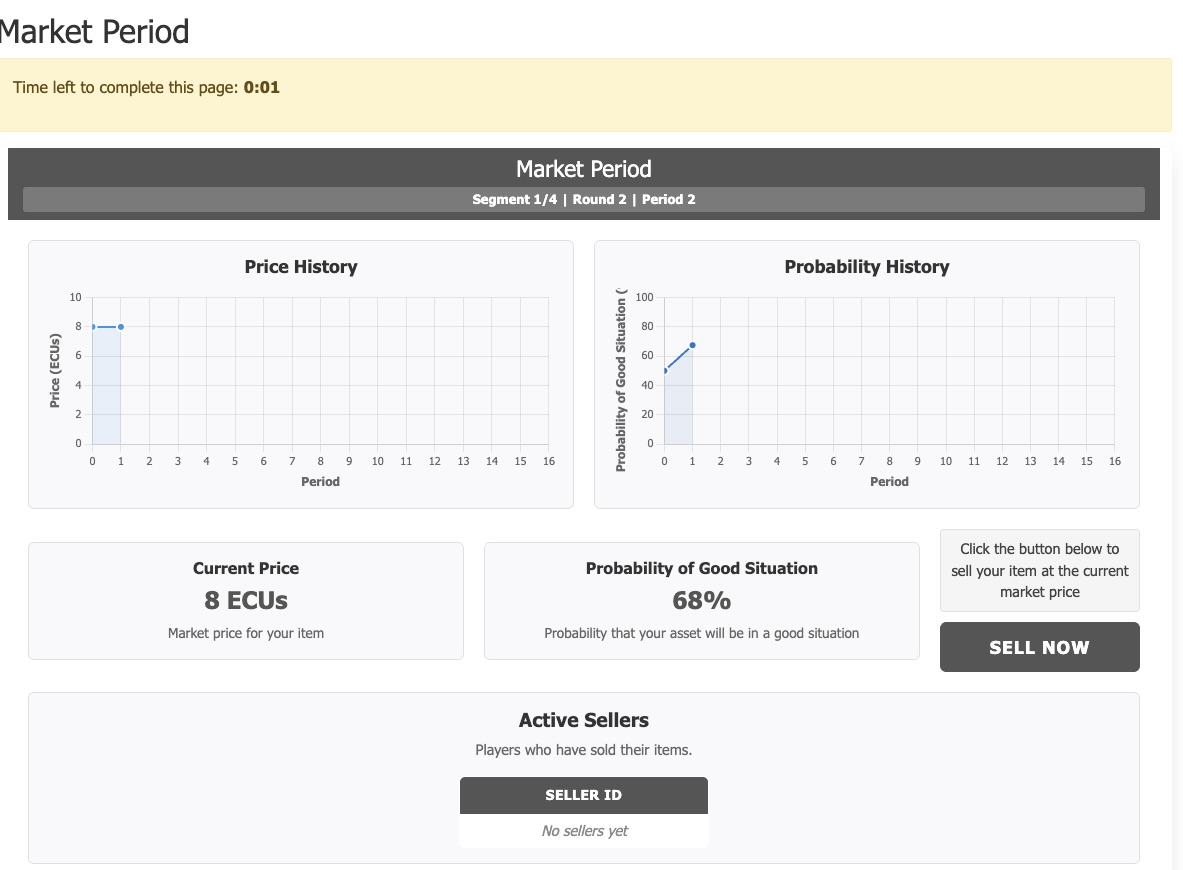
\includegraphics[width=0.85\linewidth]{interface.jpeg}
\end{center}
\end{frame}


\begin{frame}{Treatment Comparison: A Liquidation Example}
Suppose at time $t-1$, no one has sold. In period $t$, A and B both sell.

\vspace{0.3cm}
\textbf{Treatment 1 (Random):}
\begin{itemize}
    \item A gets $p_4 = 8$ or $p_3 = 6$ (50/50); B gets the other
\end{itemize}

\textbf{Treatment 2 (Average):}
\begin{itemize}
    \item Both get $\bar{p} = (8+6)/2 = 7$
\end{itemize}

\vspace{0.3cm}
Key properties:
\begin{itemize}
    \item $E(P_1) = E(P_2)$ (same expected payoff)
    \item $Var(P_1) \geq Var(P_2)$ (Treatment 2 removes payoff uncertainty)
    \item $Var(P_2) = 0$ when multiple sell simultaneously
\end{itemize}
\end{frame}

%%%%%%%%%%%%%%%%%%%%%%%%%%%%%%%%%%%%%
% SUMMARY STATISTICS
%%%%%%%%%%%%%%%%%%%%%%%%%%%%%%%%%%%%%

\begin{frame}{Subject Pool}
\begin{center}
\scalebox{0.72}{
\begin{tabular}{lcccc}
\toprule
 & Range & Full Sample & Treatment 1 & Treatment 2 \\
\midrule
  $N$ (subjects) & & 96 & 48 & 48 \\
  $N$ (sessions) & & 6 & 3 & 3 \\
  Age & & 21.13 (3.23) & 21.21 (3.19) & 21.04 (3.30) \\
  Female (\%) & & 56.8 & 58.3 & 55.3 \\
\midrule
  Extraversion & [1,7] & 4.48 (1.48) & 4.31 (1.66) & 4.66 (1.26) \\
  Agreeableness & [1,7] & 4.83 (1.07) & 4.90 (1.09) & 4.77 (1.05) \\
  Conscientiousness & [1,7] & 5.57 (1.14) & 5.29 (1.13) & 5.85 (1.09) \\
  Neuroticism & [1,7] & 3.32 (1.43) & 3.49 (1.46) & 3.15 (1.38) \\
  Openness & [1,7] & 5.17 (1.12) & 5.21 (1.12) & 5.13 (1.12) \\
  Impulsivity & [1,7] & 3.09 (0.82) & 3.08 (0.79) & 3.10 (0.86) \\
  State Anxiety & [1,4] & 1.69 (0.55) & 1.65 (0.56) & 1.73 (0.55) \\
  Risk Tolerance & [0,20] & 11.80 (6.75) & 12.27 (6.44) & 11.32 (7.08) \\
\bottomrule
\end{tabular}
}
\end{center}
\vspace{-0.2cm}
{\tiny\textit{Note:} Trait values as Mean (SD). Based on 95 survey respondents.}
\end{frame}


\begin{frame}{Selling Behavior Summary}
\begin{center}
\scalebox{0.62}{
\begin{tabular}{lcccc}
\toprule
 & \multicolumn{2}{c}{Treatment 1} & \multicolumn{2}{c}{Treatment 2} \\
\cmidrule(lr){2-3} \cmidrule(lr){4-5}
 & No Chat & Chat & No Chat & Chat \\
\midrule
  Total group-rounds & 180 & 180 & 180 & 180 \\
\midrule
  Group-rounds by seller count & & & & \\
  \quad 0 sellers & 68 & 123 & 56 & 91 \\
  \quad 1 seller & 53 & 26 & 54 & 43 \\
  \quad 2 sellers & 37 & 26 & 42 & 23 \\
  \quad 3 sellers & 20 & 4 & 25 & 19 \\
  \quad 4 sellers & 2 & 1 & 3 & 4 \\
\midrule
  Avg sellers per group-round & 1.08 & 0.52 & 1.25 & 0.90 \\
  \quad Good state & 0.89 & 0.28 & 0.99 & 0.52 \\
  \quad Bad state & 1.40 & 0.70 & 1.52 & 1.23 \\
\midrule
  Avg sell period by seller position & & & & \\
  \quad 1st seller & 2.3 & 3.2 & 2.5 & 2.6 \\
  \quad 2nd seller & 4.0 & 5.5 & 3.9 & 3.8 \\
  \quad 3rd seller & 4.5 & 8.8 & 4.9 & 4.0 \\
\midrule
  Avg sell period & 2.7 & 3.9 & 3.0 & 3.0 \\
  \quad Good state & 2.5 & 3.0 & 2.7 & 2.2 \\
  \quad Bad state & 3.0 & 4.2 & 3.2 & 3.3 \\
\bottomrule
\end{tabular}
}
\end{center}
\end{frame}


%%%%%%%%%%%%%%%%%%%%%%%%%%%%%%%%%%%%%
% MAIN RESULTS
%%%%%%%%%%%%%%%%%%%%%%%%%%%%%%%%%%%%%

%%%%%%%%%%%%%%%%%%%%%%%%%%%%%%%%%%%%%
% TOBIT: GROUP-ROUND LEVEL
%%%%%%%%%%%%%%%%%%%%%%%%%%%%%%%%%%%%%

\begin{frame}{Group-Round Level (Tobit)}
\vspace{-0.3cm}
\begin{equation*}
    n\_sellers^*_{gr} = \beta_0 + \beta_1 \text{BadState}_r + \beta_2 \text{Tr2}_g + \textstyle\sum_{s=2}^{4} \gamma_s \mathbf{1}[\text{Seg}\!=\!s] + \delta \text{Round}_r + \varepsilon_{gr}
\end{equation*}
\vspace{-0.4cm}
\begin{center}
\scalebox{0.72}{
\begingroup
\centering
\scriptsize
\begin{tabular}{lcc}
   \tabularnewline \midrule \midrule
   Dependent Variable: & \multicolumn{2}{c}{Number of Sellers in Round}\\
   Model:               & (1)  & (2)\\
   \midrule
   \emph{Variables}\\
   Constant                  & 0.8740$^{***}$ & 0.5603$^{**}$\\
                             & (0.2694) & (0.2664)\\
   Bad state                 &  & 0.9827$^{***}$\\
                             &  & (0.1551)\\
   Treatment 2               & 0.5388$^{**}$ & 0.4952$^{**}$\\
                             & (0.2242) & (0.2168)\\
   Segment 2                 & -0.3344 & -0.3539\\
                             & (0.2597) & (0.2486)\\
   Segment 3                 & -0.9845$^{***}$ & -1.0700$^{***}$\\
                             & (0.3218) & (0.3144)\\
   Segment 4                 & -1.1254$^{***}$ & -1.2829$^{***}$\\
                             & (0.3159) & (0.3027)\\
   Round                     & -0.0569$^{**}$ & -0.0738$^{***}$\\
                             & (0.0274) & (0.0256)\\
   \midrule
   \emph{Fit statistics}\\
   Observations              & 720 & 720\\
   Log-likelihood            & -998.8 & -975.3\\
   \midrule \midrule
   \multicolumn{3}{l}{\emph{Cluster-robust standard errors clustered at the group level (session $\times$ segment $\times$ group, global\_group\_id) in parentheses}}\\
   \multicolumn{3}{l}{\emph{Signif. Codes: ***: 0.01, **: 0.05, *: 0.1}}\\
\end{tabular}
\par\endgroup


}
\end{center}
\end{frame}


\begin{frame}{Tobit Takeaways}
\begin{itemize}
    \item \textbf{Treatment 2} (average liquidation) \textit{increases} sellers by $\approx 0.5$ per group-round
    \begin{itemize}
        \item Contradicts H1 --- pooling payoffs does not reduce runs
    \end{itemize}
    \item \textbf{Chat segments} (3 \& 4) significantly decrease sellers by $\approx 1.1$--$1.3$
    \begin{itemize}
        \item Supports H2 --- communication reduces market runs
    \end{itemize}
    \item \textbf{Bad state} increases sellers by $\approx 1.0$ (participants understood signals)
    \item \textbf{Round} has a negative effect: learning within segments
\end{itemize}
\end{frame}

%%%%%%%%%%%%%%%%%%%%%%%%%%%%%%%%%%%%%
% RANK-ORDERED LOGIT: GROUP-ROUND LEVEL
%%%%%%%%%%%%%%%%%%%%%%%%%%%%%%%%%%%%%

\begin{frame}{Selling Position (Rank-Ordered Logit)}
\vspace{-0.2cm}
\begin{equation*}
    \lambda_i(t \mid s) = \lambda_{0s}(t) \exp\bigl(
    \boldsymbol{\beta}_{\text{emo}}^{\prime} \mathbf{Emotion}_i + \boldsymbol{\beta}_{\text{demo}}^{\prime} \mathbf{Demo}_i
     + \boldsymbol{\beta}_{\text{trait}}^{\prime} \mathbf{Trait}_i \bigr)
\end{equation*}

\begin{itemize}
    \item Stratified at session-segment-group-round level
    \item Absorbs round, segment, and treatment effects
    \item Isolates emotional and personality trait effects
    \item Coefficients: log-hazard ratios (positive $=$ earlier selling)
    \item Two samples: Full (sellers + non-sellers) and sellers only
\end{itemize}
\end{frame}


\begin{frame}{Rank-Ordered Logit: Emotions}
\begin{center}
\scalebox{0.65}{
\begin{tabular}{l*{4}{>{\centering\arraybackslash}p{1.8cm}}}
   \toprule
   & \multicolumn{2}{c}{Full Sample} & \multicolumn{2}{c}{Sellers Only} \\
   \cmidrule(lr){2-3} \cmidrule(lr){4-5}
   & (1) & (2) & (3) & (4) \\
   \midrule
   Fear          & $-$0.006 & 0.006 & $-$0.183 & 0.022 \\
                 & (0.026) & (0.024) & (0.124) & (0.087) \\
   Anger         & $-$0.015 & $-$0.016$^{*}$ & $-$0.124 & 0.000 \\
                 & (0.009) & (0.009) & (0.235) & (0.235) \\
   Contempt      & $-$0.002 & $-$0.002 & 0.042 & 0.034 \\
                 & (0.012) & (0.013) & (0.045) & (0.045) \\
   Disgust       & 0.007 & 0.005 & 0.173$^{***}$ & 0.149$^{**}$ \\
                 & (0.006) & (0.007) & (0.060) & (0.059) \\
   Joy           & 0.034$^{*}$ & 0.031 & $-$0.247$^{***}$ & $-$0.215$^{**}$ \\
                 & (0.019) & (0.020) & (0.086) & (0.096) \\
   Sadness       & $-$0.007 & $-$0.005 & $-$0.037 & 0.009 \\
                 & (0.010) & (0.010) & (0.055) & (0.059) \\
   Surprise      & $-$0.016 & $-$0.018 & 0.238$^{*}$ & 0.079 \\
                 & (0.028) & (0.026) & (0.128) & (0.073) \\
   Engagement    & 0.016 & 0.009 & 0.135$^{**}$ & 0.087 \\
                 & (0.018) & (0.017) & (0.061) & (0.065) \\
   Valence       & $-$0.055$^{**}$ & $-$0.049$^{**}$ & 0.130 & 0.122 \\
                 & (0.024) & (0.024) & (0.104) & (0.108) \\
   \bottomrule
   \multicolumn{5}{l}{\scriptsize\emph{Log-hazard ratios, z-scored. SE clustered at player level. ***: 0.01, **: 0.05, *: 0.1}} \\
\end{tabular}
}
\end{center}
\end{frame}


\begin{frame}{Rank-Ordered Logit: Emotions --- Takeaways}
\begin{itemize}
    \item \textbf{Disgust}: significant positive predictor among sellers
    \begin{itemize}
        \item May operate like anger/fear --- pessimism or desire to punish
    \end{itemize}
    \item \textbf{Joy}: positive in full sample, but \textit{negative} among sellers
    \begin{itemize}
        \item Sarcastic joy cannot be distinguished by facial reading software
    \end{itemize}
    \item \textbf{Valence}: overall positivity $\rightarrow$ later selling in full sample
    \begin{itemize}
        \item Captures non-sarcastic piece of joy reading
    \end{itemize}
    \item \textbf{Engagement}: significant among sellers (more attentive $\rightarrow$ more sensitive to downward updates)
\end{itemize}
\end{frame}


\begin{frame}{Rank-Ordered Logit: Personality Traits}
\begin{center}
\scalebox{0.75}{
\begin{tabular}{l*{2}{>{\centering\arraybackslash}p{2.5cm}}}
   \toprule
   & Full Sample (2) & Sellers Only (4) \\
   \midrule
   Extraversion       & $-$0.011 & $-$0.010 \\
                      & (0.029) & (0.060) \\
   Agreeableness      & $-$0.030 & $-$0.150$^{***}$ \\
                      & (0.025) & (0.056) \\
   Conscientiousness  & 0.090$^{**}$ & 0.297$^{***}$ \\
                      & (0.045) & (0.082) \\
   Neuroticism        & 0.038$^{*}$ & $-$0.028 \\
                      & (0.023) & (0.051) \\
   Openness           & 0.023 & 0.037 \\
                      & (0.016) & (0.034) \\
   Impulsivity        & 0.017 & 0.049 \\
                      & (0.032) & (0.059) \\
   State anxiety      & 0.052$^{***}$ & 0.162$^{***}$ \\
                      & (0.019) & (0.044) \\
   Risk tolerance     & $-$0.048$^{*}$ & 0.044 \\
                      & (0.026) & (0.046) \\
   \bottomrule
   \multicolumn{3}{l}{\scriptsize\emph{Log-hazard ratios, z-scored. SE in parentheses. ***: 0.01, **: 0.05, *: 0.1}} \\
\end{tabular}
}
\end{center}
\end{frame}


\begin{frame}{Rank-Ordered Logit: Traits --- Takeaways}
\begin{itemize}
    \item \textbf{Conscientiousness} \& \textbf{anxiety}: increase selling hazard
    \begin{itemize}
        \item Effects amplify $\approx 3\times$ in sellers-only subsample
    \end{itemize}
    \item \textbf{Agreeableness}: decreases hazard among sellers (supports H3)
    \item \textbf{Neuroticism}: marginally significant in full sample (negativity bias)
    \item \textbf{Risk tolerance}: marginally decreases hazard in full sample (supports H3)
    \item Round, segment, treatment absorbed by strata
\end{itemize}

\vspace{0.3cm}
\begin{center}
\scalebox{0.70}{
\begin{tabular}{l*{2}{>{\centering\arraybackslash}p{2.0cm}}}
   \toprule
   & Full Sample & Sellers Only \\
   \midrule
   Observations  & 2,845 & 486 \\
   Strata        & 720 & 202 \\
   Concordance   & 0.670 & 0.688 \\
   \bottomrule
\end{tabular}
}
\end{center}
\end{frame}


%%%%%%%%%%%%%%%%%%%%%%%%%%%%%%%%%%%%%
% COX SURVIVAL: PLAYER-PERIOD LEVEL
%%%%%%%%%%%%%%%%%%%%%%%%%%%%%%%%%%%%%

\begin{frame}{Player-Period Level (Cox Survival)}
\vspace{-0.2cm}
\begin{equation*}
\begin{split}
    \lambda_{it}(t) = \lambda_0(t) \exp\bigl(
    & \beta_1 D_{1,it} + \beta_2 D_{2,it} + \beta_3 D_{3,it} \\
    & + \boldsymbol{\gamma}^{\prime} \mathbf{Cascade}_{it} + \beta_s \, \text{Signal}_{it} \\
    & + \boldsymbol{\beta}_{\text{emo}}^{\prime} \mathbf{Emotion}_{it} + \boldsymbol{\beta}_{\text{trait}}^{\prime} \mathbf{Trait}_i + u_i \bigr)
\end{split}
\end{equation*}

\begin{itemize}
    \item Random-effects Cox model (coxme); player random intercept
    \item Hazard ratios: $>1 \Rightarrow$ increased selling probability
    \item Period within round as survival time axis
    \item Two samples: All sellers and first sellers only
    \item Each with and without personality traits
\end{itemize}
\end{frame}


\begin{frame}{Cox Results: Cascade Effects}
\begin{center}
\scalebox{0.75}{
\begin{tabular}{l*{2}{>{\centering\arraybackslash}p{2.5cm}}}
   \toprule
   & All Sellers (1) & All Sellers (2) \\
   & No Traits & With Traits \\
   \midrule
   1 prior sale              & 0.815 & 0.824 \\
                             & (0.126) & (0.127) \\
   2 prior sales             & 0.234$^{***}$ & 0.241$^{***}$ \\
                             & (0.075) & (0.078) \\
   3 prior sales             & 0.049$^{***}$ & 0.050$^{***}$ \\
                             & (0.050) & (0.051) \\
   \midrule
   1 prior $\times$ 1 prev.  & 1.177 & 1.174 \\
                             & (0.210) & (0.209) \\
   2 prior $\times$ 1 prev.  & 2.807$^{***}$ & 2.791$^{***}$ \\
                             & (1.086) & (1.080) \\
   2 prior $\times$ 2 prev.  & 3.254$^{***}$ & 3.205$^{***}$ \\
                             & (1.410) & (1.388) \\
   \bottomrule
   \multicolumn{3}{l}{\scriptsize\emph{Hazard ratios. SE in parentheses. ***: 0.01, **: 0.05, *: 0.1}} \\
\end{tabular}
}
\end{center}

\begin{itemize}
    \item More cumulative sales $\rightarrow$ \textbf{lower} hazard (lower opportunity cost of holding)
    \item Sales in the \textbf{immediately prior period} $\rightarrow$ \textbf{higher} hazard
    \item Cascade/herding despite public signals and no new information
\end{itemize}
\end{frame}


\begin{frame}{Cox Results: Emotions}
\begin{center}
\scalebox{0.70}{
\begin{tabular}{l*{4}{>{\centering\arraybackslash}p{1.8cm}}}
   \toprule
   & \multicolumn{2}{c}{All Sellers} & \multicolumn{2}{c}{First Sellers} \\
   \cmidrule(lr){2-3} \cmidrule(lr){4-5}
   & (1) & (2) & (3) & (4) \\
   \midrule
   Fear          & 0.979 & 0.982 & 1.010 & 1.019 \\
                 & (0.026) & (0.027) & (0.033) & (0.033) \\
   Anger         & 0.973 & 0.969 & 0.976 & 0.975 \\
                 & (0.034) & (0.034) & (0.042) & (0.042) \\
   Contempt      & 0.986 & 0.986 & 1.008 & 1.008 \\
                 & (0.009) & (0.009) & (0.009) & (0.009) \\
   Disgust       & 0.971 & 0.971 & 1.013 & 1.013 \\
                 & (0.027) & (0.027) & (0.034) & (0.034) \\
   Joy           & 1.016$^{*}$ & 1.017$^{*}$ & 1.001 & 1.001 \\
                 & (0.009) & (0.009) & (0.011) & (0.011) \\
   Sadness       & 1.001 & 1.000 & 1.002 & 1.003 \\
                 & (0.013) & (0.013) & (0.021) & (0.020) \\
   Surprise      & 1.015 & 1.012 & 1.009 & 1.000 \\
                 & (0.019) & (0.020) & (0.025) & (0.025) \\
   Engagement    & 0.998 & 0.998 & 0.995 & 0.995 \\
                 & (0.003) & (0.003) & (0.004) & (0.004) \\
   Valence       & 0.988$^{*}$ & 0.987$^{*}$ & 1.003 & 1.003 \\
                 & (0.007) & (0.007) & (0.009) & (0.009) \\
   \bottomrule
   \multicolumn{5}{l}{\scriptsize\emph{Hazard ratios. SE in parentheses. ***: 0.01, **: 0.05, *: 0.1}} \\
\end{tabular}
}
\end{center}
\end{frame}


\begin{frame}{Cox Results: Emotions --- Takeaways}
\begin{itemize}
    \item \textbf{Joy}: marginally significant increase in selling hazard (all sellers)
    \begin{itemize}
        \item May reflect sarcastic joy detected by facial reading software
    \end{itemize}
    \item \textbf{Valence}: marginally significant decrease in selling hazard (all sellers)
    \begin{itemize}
        \item Captures non-sarcastic positivity $\rightarrow$ later selling
    \end{itemize}
    \item No individual emotion significant for first sellers
    \item Consistent with rank-ordered logit: emotions matter more at the group-round level than period-by-period
\end{itemize}
\end{frame}


\begin{frame}{Cox Results: Personality Traits}
\begin{center}
\scalebox{0.75}{
\begin{tabular}{l*{2}{>{\centering\arraybackslash}p{2.5cm}}}
   \toprule
   & All Sellers (2) & First Sellers (4) \\
   \midrule
   Extraversion       & 0.946 & 1.080 \\
                      & (0.074) & (0.091) \\
   Agreeableness      & 0.882 & 0.834 \\
                      & (0.098) & (0.098) \\
   Conscientiousness  & 1.428$^{***}$ & 1.388$^{**}$ \\
                      & (0.194) & (0.195) \\
   Neuroticism        & 1.064 & 1.059 \\
                      & (0.099) & (0.105) \\
   Openness           & 1.072 & 1.054 \\
                      & (0.106) & (0.108) \\
   Impulsivity        & 1.202 & 1.278 \\
                      & (0.194) & (0.213) \\
   State anxiety      & 1.546$^{**}$ & 1.324 \\
                      & (0.313) & (0.287) \\
   Risk tolerance     & 0.964$^{**}$ & 1.012 \\
                      & (0.016) & (0.018) \\
   \bottomrule
   \multicolumn{3}{l}{\scriptsize\emph{Hazard ratios. SE in parentheses. ***: 0.01, **: 0.05, *: 0.1}} \\
\end{tabular}
}
\end{center}
\end{frame}


\begin{frame}{Cox Results: Traits --- Takeaways}
\begin{itemize}
    \item \textbf{Conscientiousness}: 43\% increase in selling hazard, significant in both samples
    \begin{itemize}
        \item Duty to sell at the ``correct'' moment $\rightarrow$ premature selling
    \end{itemize}
    \item \textbf{State anxiety}: 55\% increase in selling hazard (all sellers)
    \begin{itemize}
        \item More sensitive to downward signal updates
    \end{itemize}
    \item \textbf{Risk tolerance}: 3.6\% decrease per unit (all sellers)
    \begin{itemize}
        \item Willing to tolerate more uncertainty about the state
    \end{itemize}
    \item All three effects consistent with rank-ordered logit and hypotheses
    \item Conscientiousness is the only trait significant for first sellers
\end{itemize}
\end{frame}


\begin{frame}{Cox Results: Controls}
\begin{center}
\scalebox{0.75}{
\begin{tabular}{l*{2}{>{\centering\arraybackslash}p{2.5cm}}}
   \toprule
   & All Sellers (2) & First Sellers (4) \\
   \midrule
   Signal            & 0.004$^{***}$ & 0.003$^{***}$ \\
                     & (0.001) & (0.001) \\
   Round             & 0.942$^{***}$ & 0.946$^{**}$ \\
                     & (0.016) & (0.022) \\
   Segment 2         & 0.847 & 0.591$^{***}$ \\
                     & (0.102) & (0.094) \\
   Segment 3 (Chat)  & 0.336$^{***}$ & 0.389$^{***}$ \\
                     & (0.044) & (0.064) \\
   Segment 4 (Chat)  & 0.329$^{***}$ & 0.402$^{***}$ \\
                     & (0.038) & (0.063) \\
   Treatment 2       & 1.140 & 0.855 \\
                     & (0.245) & (0.192) \\
   \bottomrule
   \multicolumn{3}{l}{\scriptsize\emph{Hazard ratios. SE in parentheses. ***: 0.01, **: 0.05, *: 0.1}} \\
\end{tabular}
}
\end{center}

\begin{itemize}
    \item \textbf{Signal}: strong negative effect --- participants understood signals
    \item \textbf{Chat} (Segments 3--4): $\approx 65\%$ reduction in selling hazard (supports H2)
    \item \textbf{Treatment 2}: not significant (does not support H1)
    \item \textbf{Round}: learning effect --- less selling as segment progresses
\end{itemize}
\end{frame}


\begin{frame}{Cox Model Summary}
\begin{center}
\scalebox{0.75}{
\begin{tabular}{l*{4}{>{\centering\arraybackslash}p{1.6cm}}}
   \toprule
   & \multicolumn{2}{c}{All Sellers} & \multicolumn{2}{c}{First Sellers} \\
   \cmidrule(lr){2-3} \cmidrule(lr){4-5}
   & (1) & (2) & (3) & (4) \\
   & No Traits & With Traits & No Traits & With Traits \\
   \midrule
   Observations  & 13,590 & 13,590 & 1,183 & 1,183 \\
   Events        & 659 & 659 & 467 & 467 \\
   Participants  & 95 & 95 & 83 & 83 \\
   Log-lik.      & $-$4401.0 & $-$4393.0 & $-$2227.9 & $-$2220.9 \\
   \bottomrule
\end{tabular}
}
\end{center}
\vspace{0.3cm}
\begin{itemize}
    \item Adding traits improves model fit in both samples
    \item 659 selling events across 95 participants
    \item 467 first-seller events across 83 participants (87\% were first seller at least once)
\end{itemize}
\end{frame}

%%%%%%%%%%%%%%%%%%%%%%%%%%%%%%%%%%%%%
% ADDITIONAL RESULTS
%%%%%%%%%%%%%%%%%%%%%%%%%%%%%%%%%%%%%

\begin{frame}{Result 4: Luck and Future Selling}
Does being ``unlucky'' in a liquidation event predict future selling?
\begin{equation*}
\text{Sold}_{i,g,r+1} = \sum_{k \in \{4,6,8\}} \beta_k \cdot \mathbf{1}[\text{Payoff}_{i,g,r} = k] + \gamma \cdot \text{PriorSales}_{i,g,r} + \alpha_{g \times r} + \varepsilon_{i,g,r}
\end{equation*}

\begin{columns}[T]
\begin{column}{0.55\textwidth}
\begin{itemize}
    \item Reference: Payoff = 2 (unluckiest)
    \item Group-round fixed effects
    \item Treatment 1 only (random liquidation)
\end{itemize}
\end{column}
\begin{column}{0.4\textwidth}
\vspace{-0.3cm}
\centering
\scriptsize
\begin{tabular}{@{}lc@{}}
   \midrule \midrule
   Dep.\ Var:    & Sold next round \\
   \midrule
   Payoff 4                & $-$0.035\\
                           & (0.032)\\
   Payoff 6                & $-$0.066\\
                           & (0.044)\\
   Payoff 8                & $-$0.092$^{*}$\\
                           & (0.053)\\
   Prior sales             & 0.015$^{**}$\\
                           & (0.007)\\
   \midrule
   Group-Round FE          & Yes\\
   Observations            & 416\\
   R$^2$                   & 0.420\\
   \midrule \midrule
   \multicolumn{2}{l}{\tiny\emph{***: 0.01, **: 0.05, *: 0.1}}\\
\end{tabular}
\end{column}
\end{columns}
\end{frame}


\begin{frame}{Result 4: Luck Takeaways}
\begin{itemize}
    \item Receiving payoff of 8 (vs.\ 2) $\rightarrow$ \textbf{9.2\% less likely} to sell next round
    \item Coefficients are \textbf{monotonically decreasing}: luckier $\rightarrow$ less likely to sell
    \item Payoffs of 4 and 6 (vs.\ 2) not individually significant
    \item \textbf{Relative income effect}: being unlucky causes more future selling, even though rounds are independent
    \item Evidence against purely rational updating
\end{itemize}
\end{frame}


%%%%%%%%%%%%%%%%%%%%%%%%%%%%%%%%%%%%%
% CONCLUSION
%%%%%%%%%%%%%%%%%%%%%%%%%%%%%%%%%%%%%

\begin{frame}{Summary of Hypothesis Tests}
\begin{center}
\begin{tabular}{lcc}
\toprule
\textbf{Hypothesis} & \textbf{Prediction} & \textbf{Evidence} \\
\midrule
H1: Average treatment & Fewer sellers & \textcolor{red}{Not supported} \\
H2: Chat treatment & Fewer sellers & \textcolor{green!50!black}{Supported} \\
H3: Conscientiousness & More sellers & \textcolor{green!50!black}{Supported} \\
H3: Anxiety & More sellers & \textcolor{green!50!black}{Supported} \\
H3: Risk tolerance & Fewer sellers & \textcolor{green!50!black}{Supported} \\
H3: Agreeableness & Fewer sellers & \textcolor{green!50!black}{Supported (sellers)} \\
H4: Disgust & More sellers & \textcolor{green!50!black}{Supported (sellers)} \\
H4: Joy & Fewer sellers & \textcolor{orange}{Mixed} \\
\bottomrule
\end{tabular}
\end{center}
\end{frame}


\begin{frame}{Conclusion}
\begin{itemize}
    \item Individual psychological factors are significant predictors of market run participation
    \item \textbf{Emotions:} Disgust increases selling; overall positivity (valence) decreases it
    \item \textbf{Traits:} Conscientiousness and anxiety increase selling; risk tolerance and agreeableness decrease it
    \item \textbf{Cascades:} Recent sales trigger panic despite providing no new information
    \item \textbf{Luck:} ``Unlucky'' payoffs increase future selling (relative income effect)
    \item \textbf{Communication:} Chat reduces market runs significantly
\end{itemize}

\vspace{0.3cm}
\textbf{Policy implications:}
\begin{itemize}
    \item Communication increases market stability
    \item Language that avoids stimulating negative emotions may prevent runs
    \item Prices are not solely driven by fundamentals
\end{itemize}
\end{frame}


\begin{frame}{Future Work}
\begin{itemize}
    \item Survey professional traders on personality traits
    \begin{itemize}
        \item Use sufficient statistics to compare with experimental panic sellers
    \end{itemize}
    \item Test interventions to mitigate negative emotional reactions
    \item Semi-private signals for a more realistic market setting
    \begin{itemize}
        \item Sales would then provide additional information beyond price changes
    \end{itemize}
\end{itemize}

\vspace{1cm}
\centering
\Large Thank you!
\end{frame}


\end{document}
